\documentclass{article}
\usepackage[preprint,nonatbib]{neurips_2026}
\usepackage[T1]{fontenc}
\usepackage{amsmath,amssymb,graphicx,booktabs,url}
\usepackage[hidelinks]{hyperref}
\newcommand{\BestVal}{2294.26}
\newcommand{\BestEpoch}{26}
\newcommand{\FIDValue}{196.60}
\newcommand{\ISValue}{1.769}
\newcommand{\TrainMinutes}{6.3}
\newcommand{\FirstTrain}{2582.65}
\newcommand{\LastTrain}{2390.55}
\newcommand{\LastKL}{22.48}
\newcommand{\VisualObservation}{The samples show coarse lung and torso silhouettes with variation in brightness and width, but substantial blur and missing fine anatomical detail.}

\title{Chest X-Ray Generation with a VAE}
\author{ECE 285 --- Homework 1}
\begin{document}
\maketitle
\begin{abstract}
A PyTorch variational autoencoder (VAE) learns to generate $64\times64$ chest X-rays from the assigned Kaggle dataset. A 30-epoch CPU run selects epoch \BestEpoch\ with validation loss \BestVal\ nats/image. Prior samples obtain Inception Score \ISValue\ and 2048-feature FID \FIDValue. These ImageNet-based metrics do not establish clinical validity.
\end{abstract}

\section{Model and objective}
Following Kingma and Welling [1], four ReLU convolutional layers (kernel 4, stride 2, padding 1; channels 32, 64, 128, 256) encode images into $256\times4\times4$ features. Linear heads predict the mean $\mu$ and log variance $\ell$ of a 64-dimensional Gaussian. A linear layer and four transposed convolutions (channels 128, 64, 32, 1) decode samples to sigmoid grayscale intensities. This unconditional model has 2,168,641 parameters and is trained from scratch.
\begin{equation}
 z=\mu+\exp(\ell/2)\odot\epsilon,\quad \epsilon\sim\mathcal{N}(0,I),\qquad
 \mathcal{L}=\sum_{p}\mathrm{BCE}(x_p,\hat{x}_p)
 +\frac12\sum_j(\mu_j^2+e^{\ell_j}-1-\ell_j).
\end{equation}
The pixel and latent sums are averaged over the batch ($\beta=1$). BCE on continuous gray values is a soft-target reconstruction surrogate; no continuous-image likelihood claim is made. New images use $z\sim\mathcal{N}(0,I)$, independently of any input image.

\section{Data and training settings}
Only one canonical copy of the assigned Kaggle archive [2] is used; duplicate directory trees are excluded. The original splits contain 5,216 training, 16 validation, and 624 test images. NORMAL and PNEUMONIA images are pooled without label balancing. Each image is converted to grayscale, resized directly to $64\times64$ with PIL bilinear interpolation, and scaled to $[0,1]$; no augmentation is applied. This direct resize can distort aspect ratio.

Adam uses learning rate $10^{-3}$, momentum $(0.9,0.999)$, batch size 64, and 30 epochs, with seed 285 and six CPU threads. Fixed-noise validation selects epoch \BestEpoch; test data are excluded from selection. Total run time is \TrainMinutes\ minutes.

\begin{figure}[!ht]
\centering
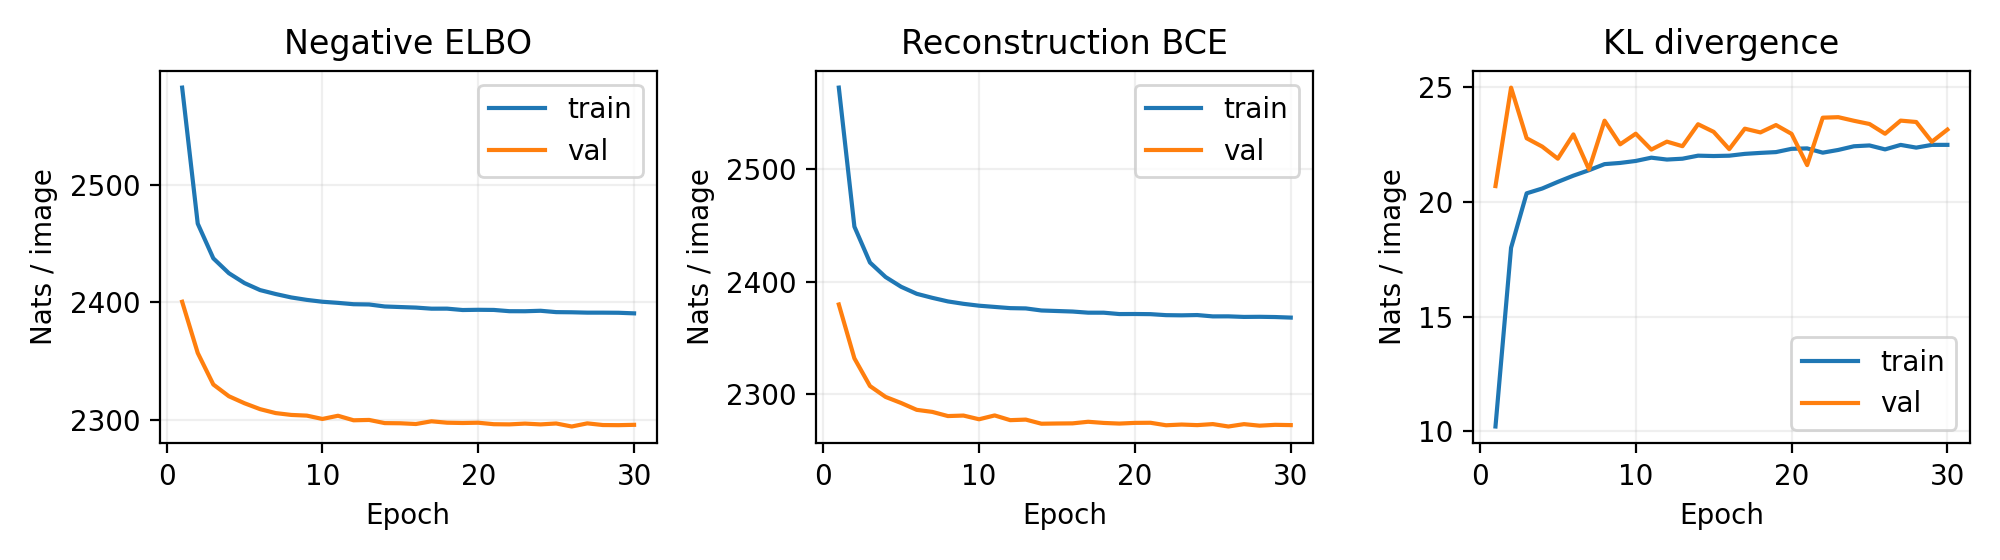
\includegraphics[width=0.88\linewidth]{images/loss_curves.png}
\caption{Training/validation loss components (nats/image) over 30 epochs.}
\end{figure}
\newpage

\section{Generation and quantitative evaluation}
\begin{figure}[!ht]
\centering
\begin{minipage}[c]{0.38\linewidth}
\centering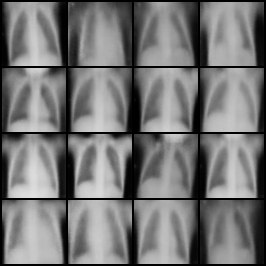
\includegraphics[width=\linewidth]{images/samples16.png}
\end{minipage}\hfill
\begin{minipage}[c]{0.58\linewidth}
\centering
\begin{tabular}{lr}
\toprule
Measurement & Result \\
\midrule
Selected epoch & \BestEpoch \\
Train loss (epoch 30) & \LastTrain \\
Best validation loss & \BestVal \\
FID (2048 features) $\downarrow$ & \FIDValue \\
Inception Score $\uparrow$ & \ISValue \\
Real / generated count & 624 / 624 \\
\bottomrule
\end{tabular}
\end{minipage}
\caption{Left: the first 16 unconditional prior samples with seed 287 from the selected model, without visual selection. Right: observed losses (nats/image) and test-set metrics. Evaluation uses a separate seed, 1285.}
\end{figure}

PyTorch-Ignite [3] accumulates FID and IS on all 624 held-out test images and 624 newly generated images. Both sets use identical uint8 quantization, gray-to-RGB channel repetition, PIL bilinear resizing to $299\times299$, and ImageNet normalization. A frozen torchvision Inception-v3 with ImageNet weights extracts pooled features and classification probabilities. No test image is used to fit the VAE or select an epoch.

FID compares the means and covariances of \emph{2048-dimensional pooled features}. This explicitly overrides Ignite's default 1000-dimensional probability representation in the assigned tutorial. The result is specific to this torchvision/PIL protocol and is not directly comparable to TensorFlow FID or Clean-FID values. IS is $\exp(\mathbb{E}_x\mathrm{KL}(p(y\mid x)\Vert p(y)))$, calculated once over the full generated set; no unmeasured split standard deviation is reported.

\section{Results and limitations}
The training objective falls from \FirstTrain\ to \LastTrain\ nats/image; the best validation objective is \BestVal. The final KL is \LastKL\ nats/image; this alone does not establish an informative or disentangled latent representation. \VisualObservation

One evaluation seed and only 624 images relative to 2048 feature dimensions make FID biased, with singular empirical covariances. ImageNet metrics cannot establish diagnostic quality. SHA-256 checks find no identical files across splits; patient independence and absence of near-duplicates remain unverified. Class imbalance, the tiny validation set, and low resolution limit interpretation. Higher resolution and patient-aware validation are untested follow-up directions.

\paragraph{Code and reproducibility.} Source code and experiment records are available at
\url{https://github.com/Raidriar7170/ece285-homework1}.
Versions: PyTorch 2.6.0, torchvision 0.21.0, Ignite 0.5.2; CPU only. The fixed display seed avoids cherry-picking.

\begin{thebibliography}{3}
\small
\bibitem{vae} D. P. Kingma and M. Welling. Auto-Encoding Variational Bayes. ICLR, 2014. \url{https://arxiv.org/abs/1312.6114}.
\bibitem{data} P. Mooney. Chest X-Ray Images (Pneumonia). Kaggle. \url{https://www.kaggle.com/datasets/paultimothymooney/chest-xray-pneumonia}.
\bibitem{ignite} PyTorch-Ignite. GAN evaluation using FID and IS. \url{https://pytorch-ignite.ai/blog/gan-evaluation-with-fid-and-is/}.
\end{thebibliography}
\end{document}
